%!TEX root = ../template.tex
%%%%%%%%%%%%%%%%%%%%%%%%%%%%%%%%%%%%%%%%%%%%%%%%%%%%%%%%%%%%%%%%%%%
%% chapter1.tex
%% UNIPD thesis document file
%%
%% Chapter with introduction
%%%%%%%%%%%%%%%%%%%%%%%%%%%%%%%%%%%%%%%%%%%%%%%%%%%%%%%%%%%%%%%%%%%

\typeout{NT FILE chapter1.tex}%

\chapter{Introduzione}
\label{cha:introduzione}

\prependtographicspath{{Chapters/Figures/Covers/}}

\section{Introduzione all’acustica nella ristorazione}

\subsection{L'importanza dell'ambiente acustico nella ristorazione}
\noindent

Negli ultimi anni, il settore della ristorazione ha visto una crescente attenzione verso l'esperienza complessiva del cliente, che va ben oltre la semplice qualità del cibo. Tra i vari fattori che influenzano questa esperienza, l'ambiente acustico gioca un ruolo cruciale, spesso sottovalutato. Il rumore di fondo in un ristorante può significativamente alterare la percezione del gusto e il godimento complessivo del pasto. \cite{castro2016percezione}

Studi recenti nel campo della psicoacustica hanno dimostrato come diversi livelli e tipi di suono possano influenzare la percezione del sapore e l'appetito. Tuttavia, la gestione dell'acustica in un ristorante presenta sfide non banali: mentre alcuni clienti potrebbero preferire un'atmosfera vivace, altri potrebbero desiderare un ambiente più tranquillo per una conversazione intima. \cite{rindel2019}

In questo contesto, emerge l'idea innovativa di creare microambienti sonori personalizzati all'interno dello stesso spazio ristorativo. Questa soluzione permetterebbe di adattare l'esperienza acustica alle preferenze individuali dei clienti, ottimizzando al contempo l'atmosfera generale del locale. L'avvento tecnologico offre nuove possibilità per realizzare questo concetto, aprendo la strada a una rivoluzione nell'design acustico dei ristoranti.

\subsection{L'evoluzione storica della tecnologia audio negli spazi pubblici}
\noindent

L’evoluzione delle tecnologie audio ha trasformato radicalmente la gestione dei suoni negli spazi pubblici, incluso il settore della ristorazione, consentendo il controllo e la personalizzazione dell’ambiente acustico.

L’introduzione della registrazione elettrica agli inizi del XX secolo, in particolare con lo sviluppo del microfono a carbone e dei sistemi di amplificazione a valvole, ha reso possibile la diffusione del suono su larga scala, sensibilizzando le industrie alla progettazione sonora per gli spazi aperti. In questi primi sviluppi, il focus era rivolto a una semplice amplificazione del suono, senza possibilità di personalizzazione.

Negli anni ’50, l’avvento dei riverberi artificiali ha segnato un ulteriore passo avanti, con dispositivi che simulavano le riflessioni sonore tipiche di ambienti come sale da concerto o teatri, rendendo possibile la manipolazione del suono anche in contesti meno tradizionali. Questo approccio ha gettato le basi per un uso strategico dell’acustica, anche in luoghi non esclusivamente dedicati alla musica. I riverberi meccanici, come quelli del famoso sistema Hammond, introdotti tra gli anni ’60 e ’70, hanno esteso questa capacità, rendendo possibile un’acustica di alta qualità anche in locali con limitazioni strutturali. \cite{liquidsonics_reverb, wired1997}

\begin{figure}[H]
    \centering
    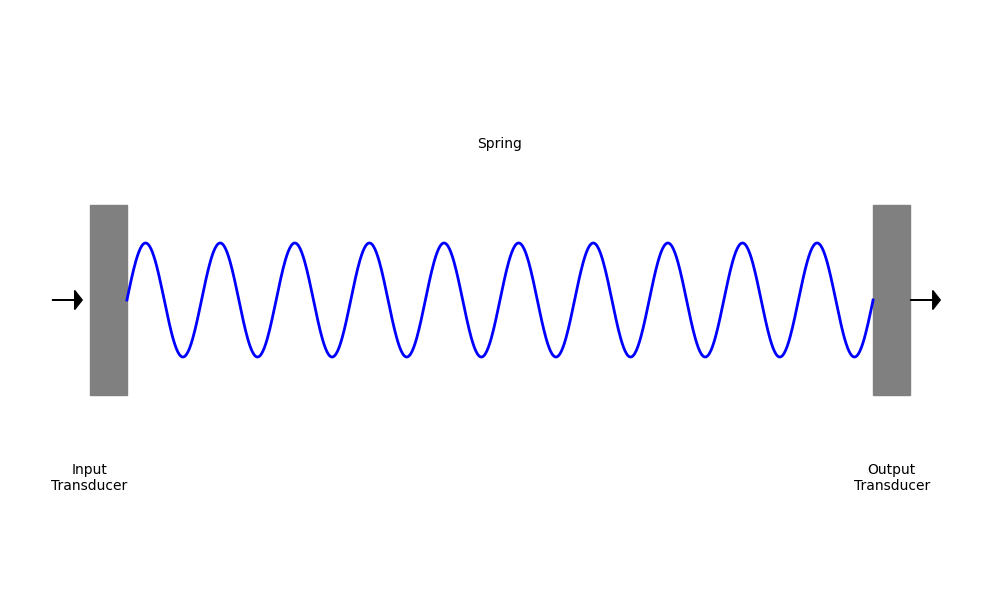
\includegraphics[width=0.6\textwidth]{Chapters/Figures/hammond_reverb.png}
    \caption{\small Rappresentazione schematica del riverbero a molla Hammond. Il diagramma illustra il principio di funzionamento attraverso i trasduttori di input e output collegati da una molla elicoidale, che converte le vibrazioni meccaniche in ritardi temporali del segnale audio.}
    \label{fig:hammond_reverb}
\end{figure}

Con la rivoluzione digitale degli anni ’80, i \gls{dsp} hanno trasformato l’elaborazione del suono, rendendo possibile il controllo dettagliato di ogni aspetto acustico: dall’equalizzazione alla gestione multi-canale. Questi processori digitali, in grado di analizzare e modificare il segnale audio in tempo reale, hanno reso l’audio un elemento dinamico e flessibile, consentendo di adattare le caratteristiche sonore alle esigenze di ogni ambiente. 

Nei ristoranti moderni, i \gls{dsp} permettono oggi di bilanciare la diffusione sonora su più aree, creando “bolle sonore” indipendenti che favoriscono un’esperienza differenziata per i clienti a seconda delle zone.

Negli ultimi decenni, con la diffusione di sistemi embedded e dispositivi programmabili a basso costo come il Raspberry Pi, la personalizzazione dell’ambiente acustico è diventata accessibile e scalabile.

Questi sistemi permettono ora di implementare configurazioni audio avanzate senza i costi elevati di infrastrutture dedicate, aprendo la strada alla gestione di ambienti multi-room sincronizzati e adattabili alle esigenze dei clienti. Nel contesto ristorativo, questa evoluzione consente di creare ambienti sonori che migliorano la percezione del gusto e favoriscono il comfort, migliorando complessivamente l’esperienza del cliente.

La sfida attuale consiste nell'integrare queste tecnologie in modo armonico, creando ambienti sonori che migliorino l'esperienza culinaria senza risultare invasivi. Questo progetto si inserisce in questo contesto, mirando a sviluppare un sistema di streaming audio personalizzato che possa contribuire a ottimizzare l'ambiente acustico nei ristoranti.

\begin{comment}
\begin{figure}[htbp]
    \centering
    \begin{tikzpicture}[mindmap, grow cyclic, every node/.style={concept, execute at begin node=\hskip0pt}, concept color=blue!40, text=black, level 1/.append style={level distance=4.5cm,sibling angle=51.4285714}, level 2/.append style={level distance=3cm}, scale=0.5, transform shape]
            \node[concept] {Audio\\Technology\\Evolution}
                child { node[alias=n1920s] {1920s\\Electrical\\Recording} }
                child { node[alias=n1950s] {1950s\\Artificial\\Reverb} }
                child { node[alias=n1960s] {1960-70s\\Electro-\\mechanical\\Devices} }
                child { node[alias=n1980s] {1980s\\Digital\\Effects} }
                child { node[alias=n1990s] {1990s\\DSP} }
                child { node[alias=n2000s] {2000s\\Spatial\\Audio} }
                child { node[alias=n2010s] {2010+\\IoT \& AI} };
            \begin{pgfonlayer}{background}
            \draw [circle connection bar] (n1920s) to (n1950s);
            \draw [circle connection bar] (n1950s) to (n1960s);
            \draw [circle connection bar] (n1960s) to (n1980s);
            \draw [circle connection bar] (n1980s) to (n1990s);
            \draw [circle connection bar] (n1990s) to (n2000s);
            \draw [circle connection bar] (n2000s) to (n2010s);
            \draw [circle connection bar] (n2010s) to (n1920s);
            \end{pgfonlayer}
    \end{tikzpicture}
    \caption{Evoluzione della tecnologia audio nel corso del tempo.}
\end{figure}

\end{comment}

\begin{figure}[H]
    \centering
    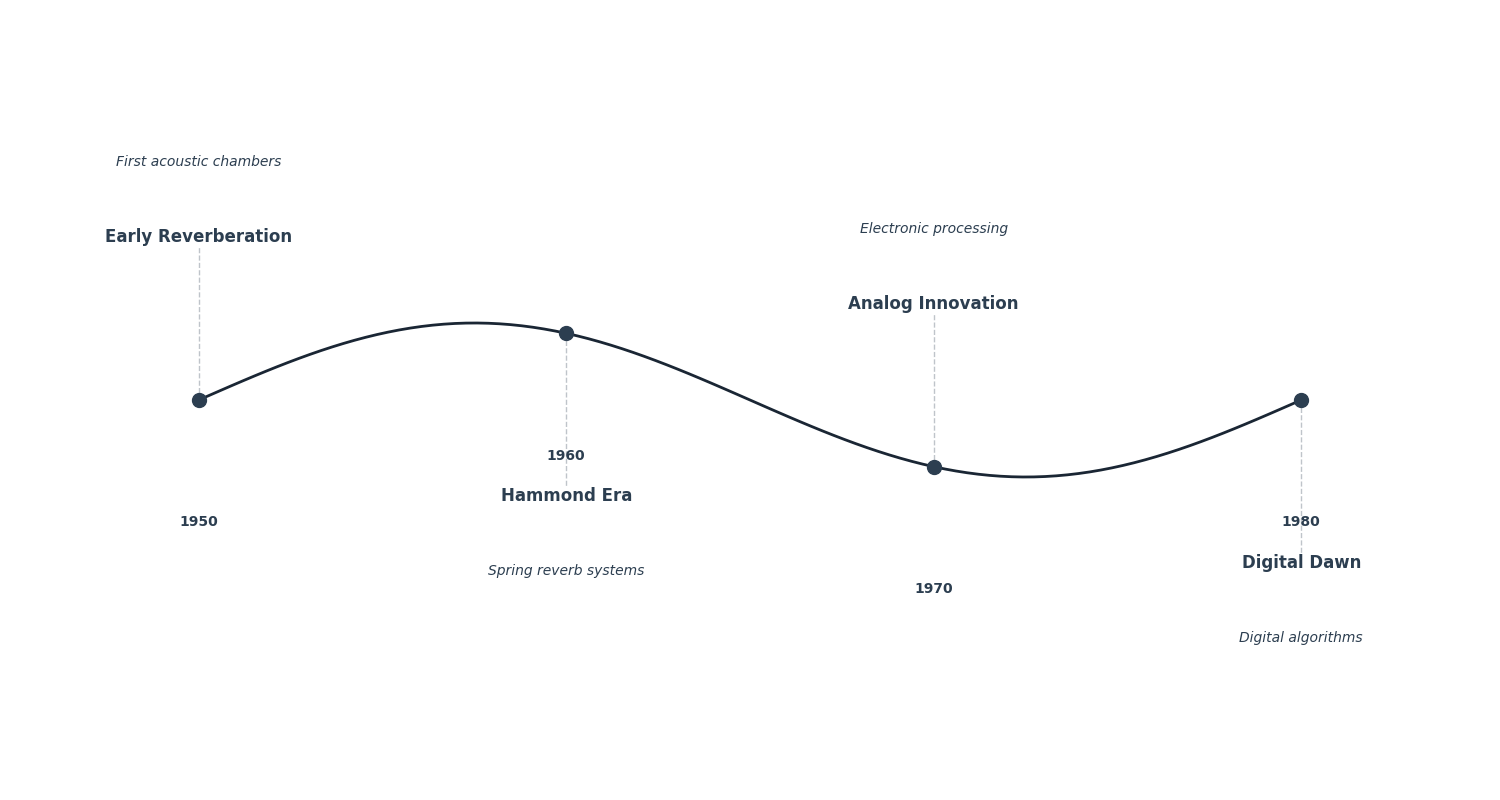
\includegraphics[width=0.9\textwidth]{Chapters/Figures/new_timeline.png}
    \caption{\small Evoluzione della tecnologia audio nel corso del tempo.}
    \label{fig:new_timeline}
\end{figure}


\section{Problematiche acustiche nei contesti ristorativi}
\noindent

La qualita dell'acustica nei ristoranti rappresenta una componente fondamentale per determinare la soddisfazione dei clienti, influenzando aspetti come la permanenza, la percezione del gusto e, piu in generale, l'esperienza complessiva. Diversi studi hanno dimostrato che l'eccesso di rumore e spesso motivo di lamentele da parte dei clienti, al pari o anche oltre la qualita del cibo e del servizio, segnalando quanto il comfort acustico sia determinante per il successo di un'attivita ristorativa. \cite{6031600}

Nei ristoranti, l'utilizzo diffuso di materiali riflettenti come vetro, piastrelle e metallo crea superfici che amplificano il rumore di fondo, prolungando il tempo di riverberazione e riducendo l'intelligibilita del parlato. Questo fenomeno acustico induce spesso i clienti ad alzare inconsciamente la voce, generando un ciclo di amplificazione del rumore che aumenta rapidamente l'intensita sonora complessiva dell'ambiente (noto come effetto Lombard). Tale contesto rende l'interazione meno agevole e contribuisce ad aumentare il livello di stress, in particolare nei periodi di picco. \cite{wilczek2020}

Oltre a compromettere la percezione sensoriale, un'acustica mal gestita limita anche la privacy acustica tra i tavoli, aspetto importante per il comfort psicologico dei clienti. La propagazione incontrollata del suono rende difficile mantenere un livello adeguato di intimità nelle conversazioni, facendo percepire l'ambiente come caotico e sovraffollato. La presenza di un ambiente eccessivamente rumoroso può portare i clienti a ridurre il tempo di permanenza e a evitare visite successive, con un impatto negativo sulla fidelizzazione. \cite{6252340}

Per migliorare la qualità del'ambiente acustico, è sempre più comune l'utilizzo di soluzioni tecnologiche avanzate come l'elaborazione del segnale digitale (\gls{dsp}) e l'impiego di materiali fonoassorbenti. Sistemi embedded come il Raspberry Pi, integrati con \gls{dsp}, consentono di modulare dinamicamente il profilo acustico, adattandolo alle diverse necessità della giornata. Questi sistemi permettono di ridurre il rumore di fondo e di migliorare la chiarezza del parlato, senza compromettere l'estetica del luogo. 

La progettazione acustica diventa così un aspetto strategico per il successo dei ristoranti moderni, influenzando non solo il comfort immediato, ma anche la probabilità di ritorno e la fidelizzazione della clientela.

\section{Obiettivi della Tesi}
\noindent

Alla luce delle problematiche acustiche descritte e dell'impatto che l'ambiente sonoro ha sull'esperienza dei clienti, questa tesi si propone di sviluppare una soluzione tecnologica avanzata e accessibile per la gestione acustica nei contesti ristorativi. L'obiettivo principale è creare un sistema integrato, basato su piattaforme embedded come il Raspberry Pi, capace di gestire in tempo reale il profilo acustico del locale.

L'obiettivo è affrontare le problematiche acustiche tipiche dei ristoranti, migliorando il comfort sonoro e creando un ambiente piacevole per i clienti. Il sistema proposto mira a gestire l'acustica del locale in modo che si adatti alle diverse esigenze degli spazi e dei momenti della giornata, contribuendo così a un'esperienza più gradevole e rilassante per tutti i presenti.